\chapter{Klasifikacijska drevesa in gozdovi}

Drevesa in gozdovi za klasifikacijo so zelo podobna tem za regresijo. Edina večja razlika je le v načinu ocenjevanja pomembnosti atributov. V tem poglavju se zato najprej seznanimo s temi metodami in jih potem uporabimo pri gradnji dreves in gozdov.

\section{Ocenjevanje pomembnosti atributov\label{c-attribute-scoring}}

Pri prav vseh praktičnih problemih uvrščanja v skupine nas zelo zanimajo atributi, ki so kar najbolj povezani z znanimi uvrstitvami primerov oziroma, kot bi temu rekli v strojnem učenju, z razredi primerov. Razkritje takih atributov nam lahko dosti pove o problemu, ki ga raziskujemo, odkrije, katere lastnosti opazovanih objektov moramo spremljati še v prihodnje oziroma so tiste, ki igrajo pomembno vlogo pri računalniški podpori odločanja. Velika večina tehnik ocenjevanj pomembnosti atributov obravnava en sam atribut ločeno od ostalih, to je, zanemari kakršnekoli medsebojne povezanosti atributov. Peščica tehnik, med katerimi bomo tu omenili eno samo, najbolj znano, pa zna razkriti pomembnost atributa tudi z ozirom na kontekst, to je, skladno z vrednostmi ostalih atributov.

Začnimo pri tehnikah, ki atribute obravnavajo vsakega zase in kontekst ostalih atributov zanemarijo. Za začetek poglejmo množico trikotnikov in kvadratov s slike~\ref{f-squares-triangles}. Želeli bi oceniti, kako dobro lahko na podlagi barve lika napovemo njegovo obliko. 

\begin{figure}[htbp]
\begin{center}
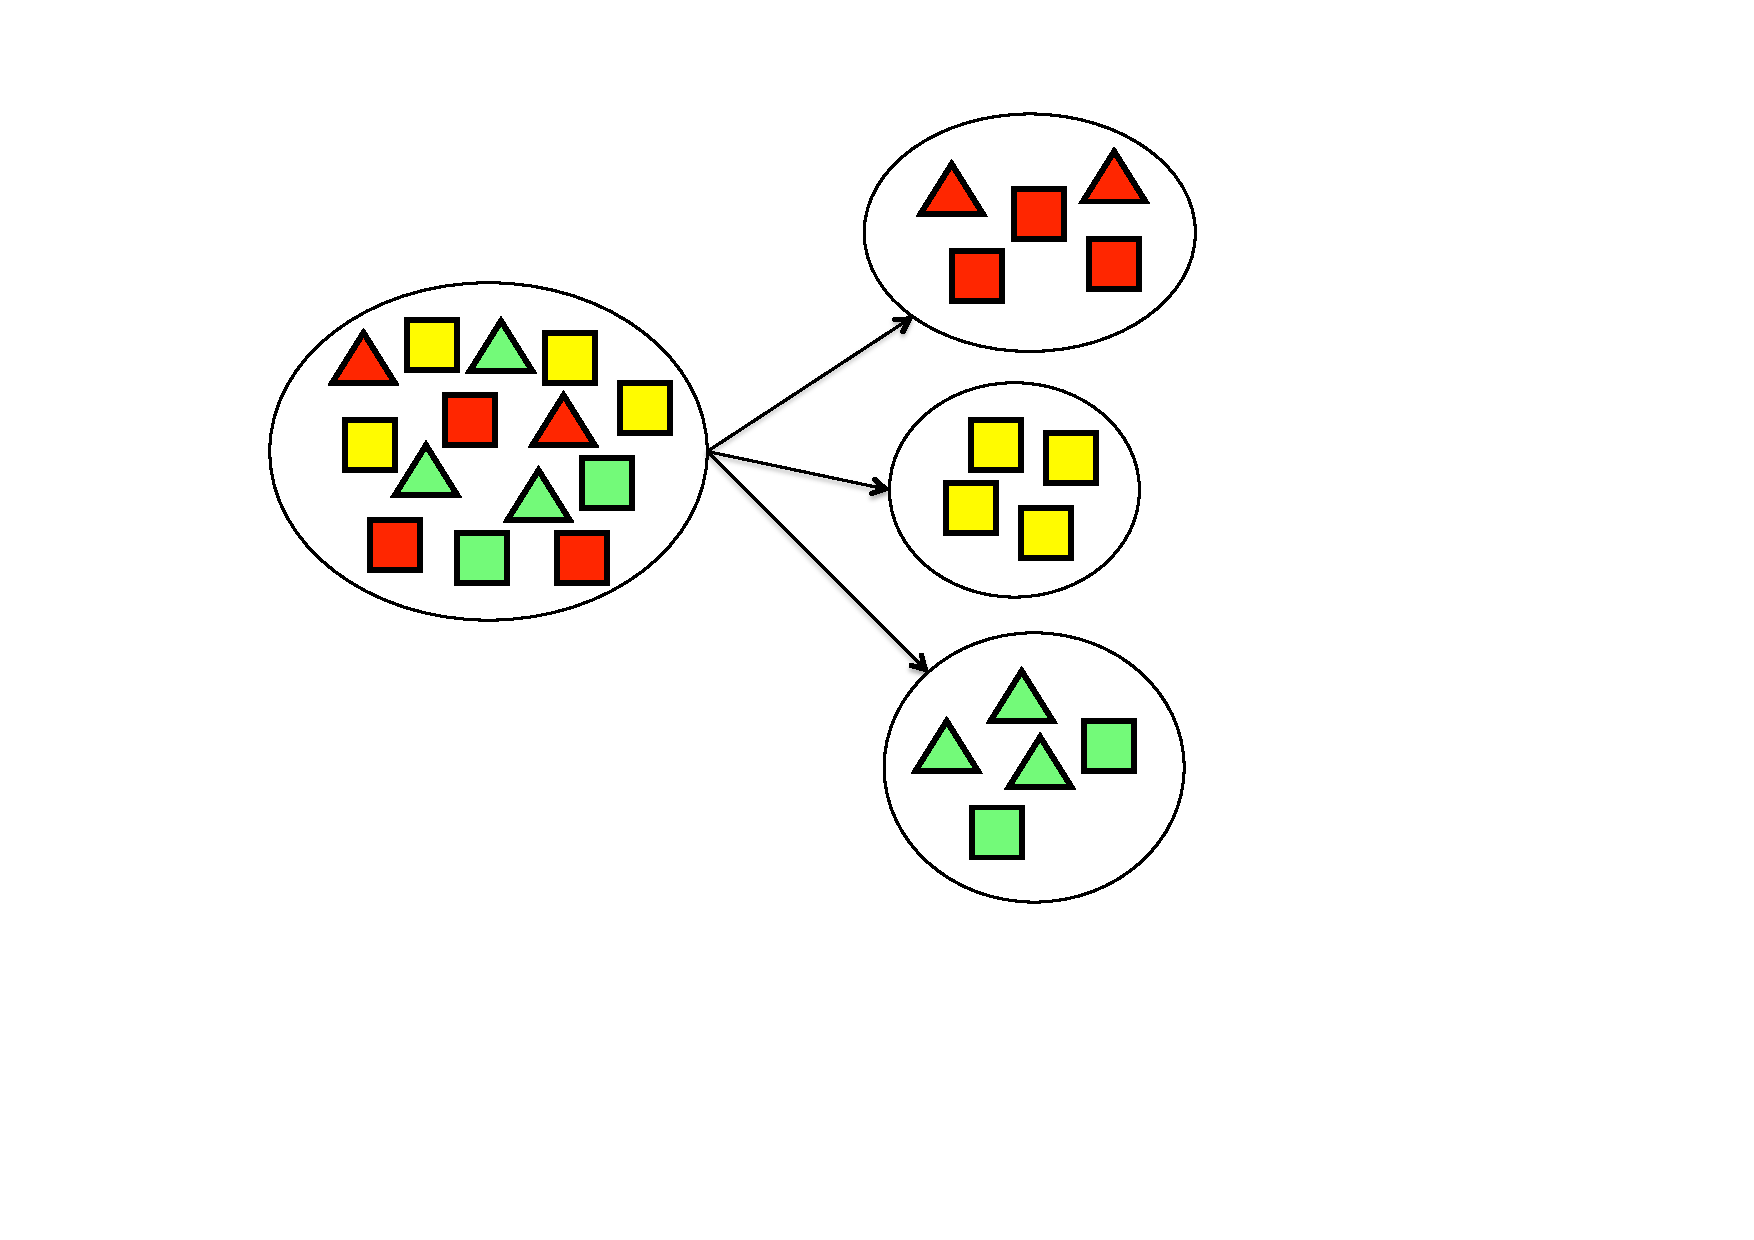
\includegraphics[width=7cm]{slike/squares-triangles.pdf}
\caption{Množica različno obarvanih kvadratov in trikotnikov (levo) in ista množica razdeljena na tri podmnožice glede na barvo likov. Vseh likov skupaj je $N=14$.}
\label{f-squares-triangles}
\end{center}
\end{figure}

\subsection{Informacijski prispevek}

Če bi bila povezanost med barvami in oblikami likov popolna, bi bile v posameznih podmnožicah na desni strani slike~\ref{f-squares-triangles} vsi liki enakih oblik. Pa niso. Pravimo, da množice niso čiste. Podmnožica rumenih likov je čista, čistočo ostalih pa bi radi zmerili. Obliko likov, naš razred, obravnavajmo kot naključno spremenljivko $C$, njene vrednosti pa označimo z $c_i$. Naša spremenljivka ima dve različni vrednosti, ``trikotnik'' in ``kvadrat''. Ocenimo še verjetnosti, da med liki iz naše celotne množice likov ($N=14$) izberemo, na primer, trikotnik. Za oceno uporabimo kar relativno frekvenco:
%
$$ P_{\triangle}={N_{\triangle} \over N} = 5/14 = 0.357 $$
%
Podobno izračunamo, da je $P_{\Box}= 0.643$. Nečistočo naše množice likov lahko ocenimo z entropijo $H$ diskretne naključne spremenljive $C$, ki je, izmerjena v bitih:
%
$$ H(C) = \sum_{i=1}^n {p(c_i)\,I(c_i)} = -\sum_{i=1}^n {p(c_i) \log_2 p(c_i)} $$
%
oziroma za naš primer:
$$ H(C) = - 0.357 \times log_2 0.357 - 0.643 \times log_2 0.643 = 0.940 $$

Ravno tako, kot za osnovno množico, lahko ocenimo nečistočo podmnožic, ki jih dobimo, ko smo like razdelili glede na njihovo barvo. Tako dobimo:
%
$$ H(C|{\rm color=red}) = -\plogp{3}{5}-\plogp{2}{5}=0.971 $$
$$ H(C|{\rm color=yellow}) = -\plogp{4}{4}-\plogp{0}{4}=0.0 $$
$$ H(C|{\rm color=green}) = -\plogp{2}{5}-\plogp{3}{5}=0.971 $$

Oceniti moramo še verjetnost, da lik pripada eni od podmnožic. Z drugimi besedami, kakšna je verjetnost, da bo naključno izbran lik iz naše osnovne množice na primer rdeč. Enostavno, 
%
$$ P_{\rm red}={N_{\rm red}\over N} = {5\over 14}=0.357$$
%
Podobno ocenimo še $P_{\rm yellow}=0.286$ in $P_{\rm green}=0.357$. Pričakovana nečistoča podmnožic, ko našo množico likov razdelimo skladno z njihovo barvno, ocenimo kot vsoto nečistoč podmnožic, ki jo utežimo z verjetnostjo, da bo lik pripadal določeni množici. Dobljeni uteženi vsoti pravimo residualna entropija:
%
$$ H_{res}=H(C|X)=\sum_{_i} p(x_i) H(C|x_i)  $$
%
in za naš primer znaša:
$$ H_{res} = 0.357 \times 0.971 + 0.286 \times 0.0 + 0.357 \times 0.971 = 0.694 $$

Pričakovana entropija, ko smo like razdelili po barvi, je torej manjša od entropije osnovne množice. Njuni razliki pravimo informacijski prispevek \angl{information gain} in z njim ocenimo, koliko informacije nam prispeva poznavanje vrednosti posameznega atributa:
$$ {\rm IG}(X) = H(C) - H(C|X) = 0.940 - 0.694 = 0.246 $$

\subsection{Relativni informacijski prispevek}

Pri atributih, ki imajo veliko zalogo vrednosti, se nam prav lahko zgodi, da nam ti primere iz osnovne množice razdelijo v zelo majhne podmnožice, morda celo take s po enim samim elementom. Entropija oziroma nečistoča slednjih je nič, a takih podmnožic si vsekakor ne želimo. Pravzaprav lahko informacijski prispevek favorizira atribute z veliko zalogo vrednosti. To ``prednost'' lahko uravnotežimo s tem, da se vprašamo, koliko informacije potrebujemo, da zvemo vrednost posameznega atributa. V našem primeru imamo med štirinajstimi liki pet rdečih, štiri rumene in pet zelenih, zato:
$$ H(X)=-\plogp{5}{14}-\plogp{4}{14}-\plogp{5}{14}=1.58 $$
%
Mero, kjer vrednost zgornjega izraza uporabimo za uravnoteženje informacijskega prispevka, imenujemo relativni informacijski prispevek \angl{information gain ratio}:
%
$$ {\rm IGR}(X) = {{\rm IG}(X)\over H(X)} $$
V našem primeru je relativni informacijski prispevek barve likov enak $0.246/1.58=0.156$.

Predlagano uravnoteženje ni edini način, da izenačimo ocene za atribute, ki imajo (zelo) različno število vrednosti. Morda bolj naravna, a računsko zahtevnejša je tehnika, ki uporablja permutacijski test in jo omenjamo v nadaljevanju.

\subsection{Mera nečistoče po Giniju}

Prikladna mera nečistoče je tudi ginijev indeks:
$$ {\rm Gini}(C)=\sum_{i}p(C=c_i)\times (1-p(C=C_i)) = 1 - \sum_i [p(C=c_i)]^2 $$
Ta ocena enaka nič za čiste množice, torej množice, kjer vsi primeri pripadajo istemu razredu, in višje vrednosti pri množicah primerov, ki pripadajo različnim razredom. Nečistoča po Giniju pove, kako pogosto bi bil za naključno izbran primer napačno napovedan razred, ki bi ga uteženo naključno napovedali iz dane porazdelitve razredne spremenljivke.

\subsection{Permutacijski test}

Pri merah, kot je večina zgornjih, včasih le težko ločimo med informativnimi in neinformativnimi atributi. Pri kakšni vrednosti mere postaviti mejo? Še težje se odločimo, če uporabljamo različne mere, kjer bi za vsako morali poznati njene statistične lastnosti. Je vrednost ocene ReliefF, ki je enaka $0.42$, dovolj visoka, da razglasimo, da je atribut informativen. Kaj pa $0.12$? Pa $0.06$? Dobro bi bilo vedeti, ali so vrednosti teh ocen pozitivne zaradi resničnih zakonitosti v podatkih ali pa smo jih dobili po naključju. Še posebej bodo ta vprašanja zanimiva za probleme, kjer je primerov malo, atributov pa veliko. 

Ocene informativnosti atributov, ki jih dobimo za vsakega od atributov, lahko primerjamo z njihovimi ničelnimi porazdelitvami, ki bi jih dobili, če bi informativnosti ocenjevali na naključno pridobljenih podatkih. Za slednje bo za nekontekstne mere dovolj premešati vrednosti razredne spremenljivke, za ReliefF ali podobne pa bo potrebno premešati celotno tabelo podatkov tako, da bomo premešali vrednosti v vsaki koloni (po atributu, torej) in na ta način ``pokvarili'' morebitni kontekst.

Za naključno premešanje razredne spremenljivke nam lahko služi spodnji razred v Pythonu. Ta si ob inicializaciji zapomni tudi izvorno uvrstitev razredov, ki jo lahko uporabi za vzpostavitev začetnega stanja. Razred je implementiran tako, da podatke ne podvaja, zapomni pa si samo vektor razredov.

\begin{python}
import random

class PermuteClass:
    """Permute the class column of the data, can also restore to original."""
    def __init__(self, data):
        self.c_vals_backup = [d.get_class() for d in data]
        self.c_vals = [d.getclass() for d in data]
    def __call__(self, data):
        random.shuffle(self.c_vals)
        for d, c in izip(data, self.c_vals):
            d.set_class(c)
    def restore(self, data):
        for d, c in izip(data, self.c_vals_backup):
            d.set_class(c)
\end{python}

Razred za premešanje vrednosti razredne spremenljivke uporablja spodnja koda, ki za vsak atribut v podatkih zgradi ničelno porazdelitev atributnih ocen.

\begin{python}
import Orange.data

epochs = 1000
alpha = 0.05
data = Orange.data.Table("voting.tab")

# define the scorer and score original data
scorer = Orange.feature.scoring.Gini()
scores = {a: scorer(a, data) for a in data.domain.attributes}

# compute null distribution, one for each attribute
null = {a:[] for a in data.domain.attributes}
permuter = PermuteClass(data)
for i in range(epochs):
    permuter(data)
    ns = [(a, scorer(a, data)) for a in data.domain.attributes]
    for a, s in ns:
        null[a].append(s)

# analyze
ps = {a: sum(1 for x in null[a] if x>scores[a])/float(epochs)
      for a in data.domain.attributes}
trash = sum(1 for p in ps.values() if p > alpha)
print "Uninformative features: %d (%d%%)" % \
    (trash, trash*100/len(data.domain.attributes))
\end{python}

Rezultat te, permutacijske analize lahko ponazorimo tudi grafično, kot to prikazuje slika~\ref{f-att-score-null}.

\begin{figure}[htbp]
\begin{center}
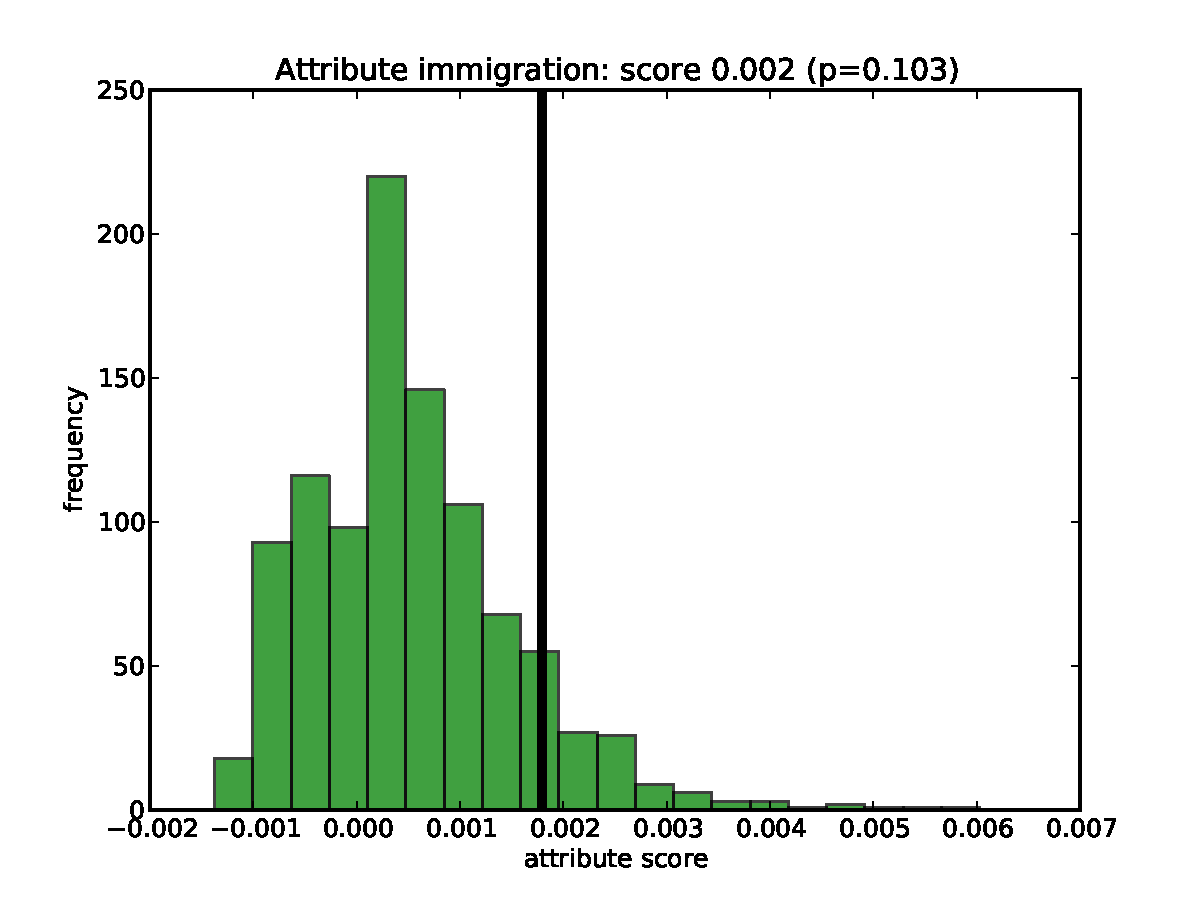
\includegraphics[width=8cm]{slike/att-score-null.pdf}
\caption{Rezultat permutacijske analize. Prikazana je porazdelitev informativnosti atributa, kot bi jo opazili, če bi bil razred primera naključen. Informativnost atributa na dejanskih, nenaključnih podatkih prikazuje vertikalna črta. Kar $10,3\%$ zmerjenih informativnost na naključnih podatkih je od te večja, zato tega atributa pri nadaljnji analizi ne bomo upoštevali.}
\label{f-att-score-null}
\end{center}
\end{figure}

Risanje grafov, kot je ta s slike~\ref{f-att-score-null}, je tipično zanimivo in informativno. Nikoli ne smemo zaupati samo golim številkam. Grafične ilustracije raznih analiz nam vedno pomagajo globlje razumeti problemsko domeno, čeprav vsi grafi niso ravno tisti, ki jih bomo vključili v naše končno poročilo. Da bo risanje takih grafov enostavneje, kodo za zgornji graf podajamo spodaj.

\begin{python}
import matplotlib.pyplot as plt

# plot score vs. null distribution for k-th worst attribute
k = 1
att, p = sorted(ps.items(), key=itemgetter(1), reverse=True)[k]
plt.close() # clear the drawing canvas
plt.hist(null[att], 20, facecolor="green", alpha=0.75)
plt.axvline(x=scores[att], color="k", linewidth=4)
plt.xlabel("attribute score")
plt.ylabel("frequency")
plt.title("Attribute %s: score %5.3f (p=%5.3f)" % (att.name, scores[att], p))
plt.savefig("att-score-null.pdf")
\end{python}

\section{Klasifikacijska drevesa}

Klasifikacijska drevesa so ena najbolj osnovnih in enostavnih orodij za gradnjo napovednih modelov pri problemih z diskretnim razredom. Ker ste ta algoritem že dobro spoznali pri uvodnih predavanjih iz umetne inteligence, tu le na kratko. Osnovna ideja algoritma je razbitje začetne množice podatkov na čim bolj (razredno) čiste podmnožice. Za razbitje uporabimo en sam atribut, razbitje pa izvedemo na podlagi njegovih vrednosti. Tako smo na sliki~\ref{f-squares-triangles} za razbitje množice likov uporabili informacijo o njihovi barvi. Ker tipično podatki vsebujejo več atributov, izberemo tistega, ki vodi k najbolj čistim podmnožicam, to je tistega, katerega informativnost je za dano množico primerov največja. V osnovnem algoritmu postopek ponavljamo na dobljenih podmnožicah vse dokler te niso čiste, ali pa dokler nismo uporabili že vseh atributov.

Rekurzivni algoritem zgradi drevo s korenom drevesa, v katerem smo imeli vse učne primere. Korenu sledijo vozlišča -- njegovi neposredni nasledniki, kjer smo primere iz osnovne množice razdelili skladno z vrednostmi najbolj informativnega atributa na podmnožice. Postopek smo ponovili vse do listov drevesa. Listom pripadajo primeri, ki izpolnjujejo pogoje oziroma imajo vrednosti atributov podane tako, kot je to zapisano na poti od lista do korena drevesa. Za vsak list lahko iz pripadajočih primerov ocenimo, kateri razred je najbolj pogost. Pravimo, da list uvršča v ta razred. Za potrebe uvrščanja se zato, glede na atributne vrednosti danega primera, sprehodimo od korena navzdol vse do lista, ki nam določa ustrezno uvrstitev.

Zgoraj smo opisali osnovni algoritem, tako imenovan algoritem ID3~\cite{} za gradnjo dreves. V izboljšanih verzijah algoritma pa lahko uporabimo tudi nekaj dodatnih trikov:
%
\begin{description}
\item[Obravnava zveznih atributov.] Te v danem vozlišču nadomestimo z binarnim atributom tako, da poiščemo mejo $t_X$, kjer skupina primerov razpade na skupino, kjer je $X<t_X$ in kjer je $X>=t_X$. Mejo $t_X$ izberemo tako, da vrednosti tega atributa, ki jih uporabljajo primeri, za katere iščemo razbitje, uredimo in preiščemo vse točke na sredini med dvemi zaporednimi vrednostmi. Izberemo tako mejno vrednost, kjer je informativnost (ocena) dobljenega binarnega atributa najvišja. Postopek imenujemo tudi kategorizacija oz. diskretizacija atributa, in je lahko primeren za predobdelavo celotne množice učnih primerov pri situacijah, kjer uporabljene metode ne znajo neposredno uporabiti zveznih atributov.

\item[Obravnava neznanih vrednosti atributov pri gradnji drevesa.] Te lahko preprosto zanemarimo oziroma jih ne upoštevamo pri ocenjevanju verjetnosti. Lahko pa jih upoštevamo tako, da ocenimo verjetnosti posameznih vrednosti in primere z neznanimi vrednostmi ustrezno ``razpršimo'' po podmnožicah.

\item[Neznane vrednosti atributov in uvrščanje.] Pri uvrščanju primerov, pri katerih nekateri atributi nimajo danih vrednosti (pravimo, da so te vrednosti neznane), lahko naletimo na vozlišče, ki zahteva poznavanje enega od teh atributov. Uvrstitev poiščemo tako, da se spustimo po vseh njegovih vejah in v vsaki poiščemo ustrezni razred, ki ga utežimo z verjetnostjo vrednosti atributa v danem vozlišču. Slednjo seveda dobimo pri učenju drevesa in si jo moramo v vozlišču, za namene uvrščanja, zapomniti.

\item[Rezanje dreves.] Drevesa tipično vodijo k drobljenju oziroma fragmentaciji problemske domene. Na razred namesto iz celotne množice primerov sklepamo iz veliko manjših podmnožic, ki pa s stališča statistike niso nujno ustrezne (bi bilo prav o pravičnosti igralne kocke razmišljati že po nekaj metih?). Bolje bi zato bilo zgraditi drevesa tako, da ta ne vodijo k premajhnim množicam v listih. Postopek se imenuje rezanje dreves. Lahko ga izvajamo vnaprej (na primer, postavimo mejo za najmanjše število primerov v listih), ali pa vzvratno tako, da zgradimo drevo in potem rekurzivno odstranjujemo nezanesljiva spodnja vozlišča. Eden od znanih postopkov za slednje imenujemo rezanje z zmanjševanjem napake \angl{minimal error prunning} in temelji na spremenjenem ocenjevanju verjetnosti tako, da pri njej upoštevamo še nekaj navideznih primerov, po enega iz vsakega razreda (t.im. ocena po Laplace-u~\cite{}) ali pa $m$ primerov, ki so porazdeljeni skladno z porazdelitvijo razredov v učni množici (t.im. $m$-ocena verjetnosti~\cite{}).

\item[Združevanje vrednosti atributov.] Nekateri diskretni atributi uporabljajo lahko (zelo) veliko število vrednosti in bi njihova uporaba pri gradnji dreves lahko vodila v takojšnjo veliko razpršitev primerov. Zato raje te vrednosti uredimo v podmnožice, ki jih poiščemo tako, da ima tako dobljeni atribut največjo informativnost. Zakaj za ocenjevanje slednje osnovna mera z informacijskim prispevkom ni primerna?
\end{description}

Tehnika gradnje in uporabe klasifikacijskih dreves ima vrsto prednosti. Je sorazmerno hitra, enostavna, zna obravnavati kakršnekoli podatke, ki jih lahko zapišemo v atributni obliki, deluje tudi na zelo velikih množicah podatkov. Uvrščanje je hitro. Model je odprt, ter ga je moč enostavno vizualizirati (slika~\ref{f-titanic-tree}) in ob njem razpravljati o možnih vzorcih v podatkih, ki jih je algoritem odkril.

\begin{figure}[htbp]
\begin{center}
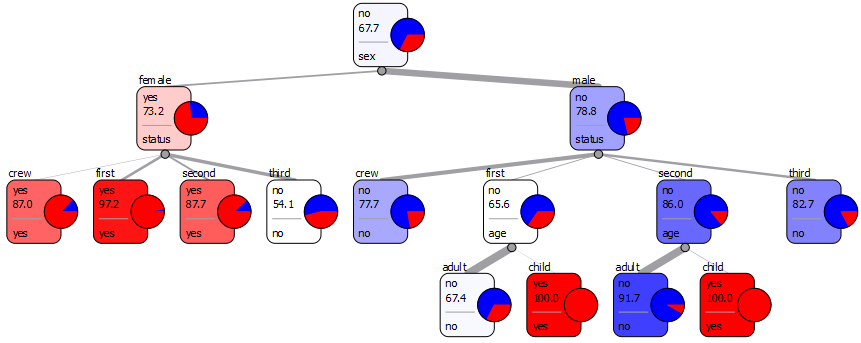
\includegraphics[width=15cm]{slike/titanic-tree.png}
\caption{Klasifikacijsko drevo zgrajeno iz podatkov o potnikih na ladji Titanic. Razred govori o preživetju nesreče. Debelina povezav med vozlišči drevesa ustreza številu primerov na teh povezavah. Barva vozlišč govori o verjetnosti prevladujočega razreda.}
\label{f-titanic-tree}
\end{center}
\end{figure}

Klasifikacijska drevesa pa imajo tudi pomanjkljivosti. O problemu fragmentacije, ki omejuje splošnost dreves in povzroči, da drevo sklepa o razredu na premajhnem vzorcu primerov, smo že govorili (kje? kdaj?). Tudi predstavljeni algoritem ne odkrije optimalnega drevesa, saj ne implementira vračanja in s tem kompleksnejše optimizacije. Drevesa so lahko izjemno velika in se lahko hitro preveč prilagodijo učnim podatkom. V splošnem drevo lahko modelira kompleksnejše povezave med primeri, na primer tudi take iz tabele~\ref{t-xor-boat}, a njih odkritje je pri uporabi univariatnih mer prepuščeno zgolj precej neverjetnemu naključju. Seveda pa lahko gradnjo dreves usmerjamo tudi s kontekstnimi merami kot je ReliefF, a s tem močno upočasnimo postopek gradnje.

Drevesa so prav tako lahko občutljiva na zelo majhne spremembe v učni množici. Prav tako se lahko zgodi, da sta dva ali več atributov med seboj zelo primerljiva po informacijski vsebini, in da majhne spremembe vplivajo na to, kateri atribut bomo izbrali. To situacijo lahko opazimo v korenu ali pa kakšnem drugem od notranjih vozlišč. V obeh primerih so lahko spremembe v strukturi drevesa izjemno velike, še posebej, če gre za vozlišče blizu vrha drevesa. Ta občutljivost je seveda nezaželena. Domenskim ekspertom bi želeli pokazati model, ki je stabilen, in se ne spreminja ob najmanjši spremembi učne množice. Izkorišča pa jo tehnika, o kateri govorimo spodaj.

\section{Naključni gozd}

Naključni gozd \angl{random forest} v uvrščanju sestavlja skupina klasifikacijskih dreves, ki pri klasifikaciji primera v razred glasuje~\cite{}. Naključni gozd napove razred, kamor primer uvršča večina klasifikacijskih dreves, ki gozd sestavlja. Najbolje bi bilo, da gozd sestavljajo drevesa, ki so med seboj različna in kjer vsako od dreves odkrije kakšen svoj, zanimiv koncept, ki se je skrival v podatkih. Podatke ti modeli osvetlijo iz različnih strani in potem skupaj o razredu glasuje. Več dreves več ve.

Taka drevesa dobimo v gozdu tako, da postopek malo ``ponaključimo''. In sicer:
\begin{enumerate}
\item Pričnemo z učno množico $D$, ki vsebuje $N$ primerov in $M$ atributov.
\item Izberemo število $m$, ki nam pove, med koliko naključno izbranih atributov iz primerov v vozliščih drevesa bomo izbrali najboljšega. Število $m$ naj bo veliko manjše od števila atributov, na primer $m=\sqrt{M}$. Izberemo tudi število dreves $K$ v gozdu, na primer $K=100$, ki ga želimo zgraditi. Nastavimo števec dreves, $i\leftarrow 1$.
\item Med $N$ primeri učne množice $D$ naključno z vračanjem izberemo novo množico primerov $D_i$ enake velikosti. To vrsto vzorčenja imenujemo metoda stremena \angl{bootstrap}. Seveda bodo v našem vzorcu posamezni primeri iz osnovne učne množice podvojeni.
\item Na množici primerov $D_i$ zgradimo klasifikacijsko drevo $T_i$, a tako, da v vsakem vozlišču naključno izberemo $m$ atributov, ki so uporabljeni v primerih vozlišča, in med njimi za delitev teh primerov izberemo najbolj informativnega upoštevaje razred primerov.
\item Če $i==K$ smo končali, sicer $i\leftarrow i+1$ in nazaj na korak 3.
\end{enumerate}

Tehnika naključnega gozda je danes ena od najbolj zanesljivih tehnik uvrščanja. Njene napovedne točnosti so tipično med najboljšimi. Tehnika podeduje vse prednosti klasifikacijskih dreves, zgubi pa možnost interpretacije modela, saj tega sedaj sestavlja vrsta modelov katerih vpliv na odločitve ni jasen in je odvisen od konteksta. Pristop v fazi gradnje modela ni med najhitrejšimi, ga pa je enostavno povzporediti.

Brieman~\cite{} je ob tem, ko je predlagal algoritem za gradnjo naključnega gozda, predlagal tudi metodo, ki oceni pomembnost, ki jo v gozdu imajo posamezni atributi pri pravilnem uvrščanju. Vsakemu vzorcu primerov $D_i$, na katerem smo zgradi drevo $T_i$,  določimo njegov komplement $D_i'=D-D_i$. Množica $D_i'$ je torej sestavljena iz primerov osnovne učne množice $D$, ki jih ni v vzorcu $D_i$ \angl{out-of-bag set}. Naj bo $C_i$ število primerov iz množice $D_i$, za katere je drevo $T_i$ pravilno napovedalo razred. Sedaj za vsak atribut $X$ premešajmo njegove vrednosti v $D_i$ in na taki, spremenjeni množici, izmerimo število pravilnih napovedi $C_{i,X}$. Pomembnost \angl{raw importance} atributa določimo kot:
%
$$ {\rm RI}(X)= {1\over K}\sum_{i=1}^K{C_i - C_{i,X}} $$

